\documentclass[12pt]{report} % Document class
% Packages
\usepackage[utf8]{inputenc} % Input encoding (UTF-8 recommended)
\usepackage[T1]{fontenc}    % Font encoding
\usepackage{lipsum}         % Lorem Ipsum dummy text
\usepackage{graphicx}       % For including images
\usepackage{float}          % For precise figure placement
\usepackage{tabularray}     % For creating tables
\usepackage{hyperref}       % For hyperlinks

\usepackage{indentfirst}    %To indent ever paragraph

\usepackage[margin=1in]{geometry} %Chnages margin

\usepackage{fancyhdr}

\pagestyle{fancy}
\fancyhf{} % Clear the header and footer

\lhead{\projectTitle}
\rhead{\reportTitle}


\fancyfoot[R]{\latestVersion}
\fancyfoot[C]{\thepage}

\newcommand*{\nsection}[1]{
    \section*{#1}
    \addcontentsline{toc}{section}{#1}
}

\usepackage{listings}

\usepackage{xcolor}

\definecolor{codegreen}{rgb}{0,0.6,0}
\definecolor{codegray}{rgb}{0.5,0.5,0.5}
\definecolor{codepurple}{rgb}{0.58,0,0.82}
\definecolor{backcolour}{rgb}{0.95,0.95,0.92}

\lstdefinestyle{mystyle}{
    backgroundcolor=\color{backcolour},   
    commentstyle=\color{codegreen},
    keywordstyle=\color{magenta},
    numberstyle=\tiny\color{codegray},
    stringstyle=\color{codepurple},
    basicstyle=\ttfamily\footnotesize,
    breakatwhitespace=false,         
    breaklines=true,                 
    captionpos=b,                    
    keepspaces=true,                 
    numbers=left,                    
    numbersep=5pt,                  
    showspaces=false,                
    showstringspaces=false,
    showtabs=false,                  
    tabsize=2
}

\lstset{style=mystyle}



\newcommand{\projectTitle}{Git Guide}
\newcommand{\reportTitle}{How to Git}
\newcommand{\latestVersion}{Version 0.0.1}


\begin{document}

% Create the title page

\clearpage
\pagenumbering{roman}
\setcounter{page}{1}

\begin{figure}
	\centering
	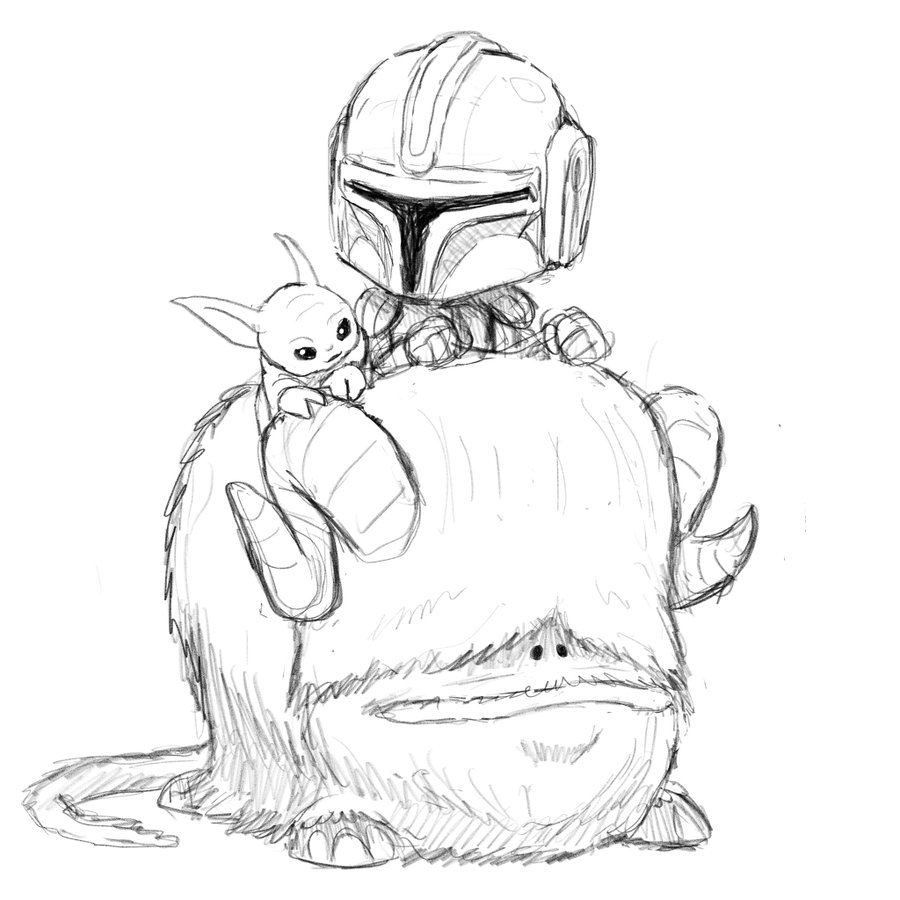
\includegraphics[width=3cm]{Fun_pics/bantha_inc.jpg}
\end{figure}

\begin{center}
	\textbf{\LARGE Bantha Inc.} \\
	\vspace{1cm}
	\Large \today \\
	\vspace{0.3cm}

	\rule{\linewidth}{0.5pt} \\
	\vspace{0.2cm}
\LARGE \projectTitle \\ \vspace{0.3cm} \large \reportTitle\\


	\vspace{0.1cm}
	\rule{\linewidth}{0.5pt} \\

	\vspace{1.5cm}

	\begin{tabular}{lr}
		\textit{Author:} & Die Go \\
	\end{tabular}

	\vspace{1cm}
	\date{}
\end{center}
\newpage

\addcontentsline{toc}{chapter}{Table of Content}
\tableofcontents



\chapter*{Revision History}
\addcontentsline{toc}{chapter}{Revision History}
\begin{center}
    \begin{tblr}{
        hlines,
        vlines,
        %row{1} = {bg=gray,fg=white},
        %row{2} = {bg=green9},
        rows = {ht=.55cm, valign=m},
        columns = {halign=c},
        %colspec = {Q[1cm,bg=gray,fg=white] XXX},} 
        %colspec = {Q[2cm] XXX},} 
        colspec = {Q[3cm] XXX},} 
        \textbf{Date} & \textbf{Version} & \textbf{Author} & \textbf{Description} \\
        08SEP2023 & 0.0.1 & Diego F. & Template Created \\
        09SEP2023 & 0.0.2 & Diego F. & Executive Summary \\
    \end{tblr}
\end{center}
\newpage




\addcontentsline{toc}{chapter}{List of Figures}
\listoffigures
\newpage

\listoftables
\addcontentsline{toc}{chapter}{List of Table}
\newpage

%Start of report
\pagenumbering{arabic}
\setcounter{page}{1}


\chapter{Introduction}
This is a guide of how to do Git. It is a really beginner thing as I will go through from how start a repo to some really cool stuff. I try to explain what stuffs does. 

\section{Initializing}

First on creating a repo, create a gitignore for it. Google the right gitignore for respective program. Like Latex and KiCad stuff. Gitignore is a file that specifies files to not be pushed to the repo. 


\begin{lstlisting}[caption={Commands for init first repo},captionpos=b,label=lst:firstRepo]
	touch .gitignore

	git init 
	
	git add .
	
	git commit -m "Msg"
	
	git remote add origin hithubURL
	
	git branch -M master
\end{lstlisting}

On the first push do:
\begin{lstlisting}[caption={First Push},captionpos=b,label=lst:firstPush]
	git push -u origin master
\end{lstlisting}


\begin{enumerate}
	\item git push: This is the main Git command used for pushing changes to a remote repository. It takes the changes you've committed locally and sends them to the specified remote repository.

	\item -u (or --set-upstream): This option is used to set up a tracking relationship between the local branch (in this case, "master") and the remote branch (in this case, "origin/master"). Setting up a tracking relationship means that in the future, when you use git push or git pull without specifying a branch name, Git will know which remote branch to push to or pull from. It's a convenient way to streamline your workflow.
	
	\item origin: This is the name of the remote repository you are pushing your changes to. "Origin" is a commonly used default name for the remote repository from which you initially cloned your local repository. You can have multiple remotes if your project requires it, and you'd use the appropriate remote name here.
	
	\item master: This is the name of the local branch that you want to push to the remote repository. In Git, "master" is a default branch name, but your project may use a different branch name as its main branch.
\end{enumerate}

So, when you run git push -u origin master, you are pushing the changes from your local "master" branch to the "master" branch in the remote repository called "origin", and you are setting up tracking so that future pushes and pulls can be done without specifying branch names if desired. 
If the remote branch is named differently then use:


\begin{lstlisting}[caption={Branch Name Change},captionpos=b,label=lst:nameChange]
	git branch -m master main
		or
	git branch -M main
\end{lstlisting}


\section{Cloning}


\chapter{Results} 

\end{document}
